%In this chapter, we start by presenting the concept of machine learning and
%supervised regression learning. Then, we discuss the details of various
%regression methods that have been explored during the course of this project.

\section{Related Works}

As discussed in Section ~\ref{sec:objectives}, our primary focus is to answer
the prediction question. However, besides the literature on using machine
learning techniques for price prediction, we first briefly review the related
works on the inference side.

\subsection{Inference}

While some research has been carried out on hotel price determinants, few
empirical investigations into the price determinants of the non-hotel
accommodation offer have been conducted.  Furthermore, most researchers
investigating the price determinant of sharing economy based accommodation have
utilized the hedonic price model.

\textcite{monty2003hedonic} assessed the price determinants of bed and breakfast
amenities and confirmed the positive effects of a hot tub, a private bath, and a
larger room on room price.  In an analysis of the impact of private tourist
accommodation facilities on prices, \textcite{portolan2013impact} found that the
presence of free parking places and sea view could be associated with a higher
room rate.  Both of the above studies recognized that location has a vital
influence on the price.

In recent years, there has been an increasing amount of literature on the price
determinants of Airbnb.  Several studies (\textcite{gutt2015sharing};
\textcite{ikkala2014defining} ) have shown that hosts who offer accommodation to
rent on Airbnb.com usually charge higher prices if their accommodation has
received high star ratings.  Using a dataset from New York City,
\textcite{li2016pros,} showed that properties managed by professional hosts earn
more in daily revenue, have higher occupancy rates, and are less likely to exit
the market than properties owned by nonprofessional hosts.
\textcite{kakar2016effects} measures the impact of information on hosts’ racial
background on Airbnb listing prices in San Francisco and found that Hispanic
hosts and Asian hosts, on average, have a lower list price relative to their
white counterparts.

\textcite{wang2017price} analyzed the Airbnb data from 33 countries and concluded
that 24 out of 25 variables within five categories (host attributes, site, and
property attributes, amenities and services, rental rules, and the number of
online reviews and ratings) are good predictors of price.  In a similar study,
\textcite{cai2019price} examines the impacts of five groups of
explanatory variables on Airbnb price in Hong Kong.


\subsection{Prediction}

To date, there is little published research on applying machine learning
techniques to predict the price of Airbnb listing.
\textcite{tang2015neighborhood} work on the task of price prediction for San
Francisco Airbnb listings by turning the regression problem into a binary
classification problem.
\textcite{li2016reasonable} has attempted to create a price prediction model for
Airbnb in different cities by using the clustering method with the distance of
the property to the city landmarks as the clustering feature.
In more recent work, \textcite{kalehbasti2019airbnb}  try to develop a reliable
price prediction model using machine learning, deep learning, and natural
language processing techniques.


This study aims to contribute to this growing area of research by utilizes a
holistic approach. In particular, the contribution is as followed:
\begin{itemize}
  \item We rely on "domain knowledge" in the feature engineering process (as
    demonstrated in Chapter ~\ref{c:data-analysis}).
  \item We make use of visualization techniques to gain insights from data.
  \item We introduce regularization techniques to improve the disadvantage of the
  traditional ordinary least square model.
  \item We present the Boosting modeling strategy, a machine learning approach
    that performs well when there are many predictors as a baseline model.
\end{itemize}

\section{Machine Learning}

Machine learning refers to creating and using models that are learned from data.
Typically, our goal will be to use existing data to develop models that we can
use to predict various outcomes for new data. Examples of machine learning
applications can be found every where. Credit card companies use it to track
fraud.  The movie recommendation system is used by Netflix to suggest movies to
subscribers. Insurance companies use it to predict the risks of potential auto,
health, and life policyholder.

Most machine learning problems fall into one of two categories: supervised or
unsupervised. The details of machine learning outline are shown in figure
\ref{fig:ml-outline}.

\begin{figure}[H]\centering
    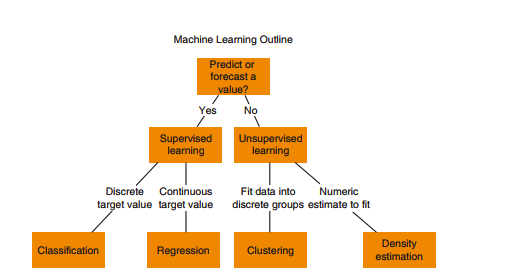
\includegraphics[width=\textwidth]{ml-outline.png}
    \caption{Machine Learning Outline}
    \label{fig:ml-outline}
    \source{\textcite{shah2020hands}}
\end{figure}

\subsection{Supervised Learning}

If our goal is to predict a specific outcome by learning how various predictors
and the response variables relate, we are dealing with \textbf{supervised
learning}. If the response variable is continuous, the problem becomes that of
\textit{regression}. If, on the other hand, the response variable is discrete,
this becomes a \textit{classification problem}. For instance, predicting the age
of a person, predicting house prices are regression problems, while predicting
the gender of a person, predicting whether a credit card transaction is
fraudulent are classification problems.

\subsection{Unsupervised Learning}
Unlike supervised learning, \textbf{Unsupervised learning} is a type of machine
learning that looks for hidden patterns in a data set with no output labels and
minimal human supervision. One of the most common unsupervised learning task is
clustering, where we group similar things together. For example, we can group
potential customers into different groups based on their characteristics, such
as income, age, gender, and shopping habits; we can group news articles into
different themes. if we are trying to explain the data by estimating underlying
processes that may be responsible for how the data is distributed, this becomes
a density estimation problem.

\section{Problem Formalization}

The problem of predicting the rental price can boil down to approximate a target
function \texttt{f} for the output variable rental price (Y) based on a set of
predictors such as \texttt{bathrooms}, \texttt{accomodates}...
We can describe the relationship between \texttt{price} (\texttt{Y}) and its
predictors $ X = (X_1, X_2, . . . , X_p) $ as followed:
\begin{eqnarray}
    Y = f(X) + \epsilon
    \label{eqn:relationship-eqn}
\end{eqnarray}

The  price of a listing can be predicted by:
\begin{eqnarray}
    \hat{Y} = \hat{f}(X)
    \label{eqn:predicted-value}
\end{eqnarray}

\section{Quantitative Measures of Performance}

Selecting the best method among many different statistical learning approaches
can be one of the practitioners' most daunting tasks.  One particular approach
may work best on a particular data set, but some other methods may perform
better on a similar but different data set.  Therefore, it is critical to select
which method produces the best results for any given data set.  To assess a
particular model's predictive performance on a given data set, we need some way
to measure how well its predictions match the observed data.
In this study, we use two standard criteria: mean squared error and coefficient
of determination.

\subsection{Mean Squared Error}
When an outcome is a number (regression problem), the most commonly used method
for characterizing a model's predictive capabilities is to use the mean squared
error (MSE), which is:

\begin{eqnarray}
    \label{eqn:mse}
    MSE = \frac{1}{n} \sum_{i=1}^{n}(y_i - \hat{f}(x_i))^2
\end{eqnarray}
where $\hat{f}(x_i)$ is the prediction that $\hat{f}$ gives for the $i^{th}$
observation. If the predicted responses are very close to the actual responses,
the MSE will be small and vice versa.

In general, we do not care how well the method works  on the training
data. Instead, we are interested in the accuracy of the test MSE predictions we
obtain when applying our method to previously unseen test data. Therefore, we
want to choose the approach that gives the lowest test MSE instead of the lowest
training MSE.

\subsection{Coefficient of Determination}
We also use the coefficient of determination ($R^2$) to measure the proportion
of the information in the data explained by the model.  For example, an $R^2$
value of 0.8 means that the model can explain  80 percent of the outcome's
variation. An $R^2$ of 1 indicates that the regression predictions perfectly fit
the data. It should be noted that $R^2$ is a measure of correlation, not
accuracy.
$R^2$ is calculated as the correlation coefficient between the
observed and predicted values and squares it:
\[ R^2 = 1 - \frac{SS_{res}}{SS_{tot}}\]
where $SS_{res}$ is the sum of squares of residuals and $SS_{tot}$ is the total
sum of squares (proportion to the variance of the data)

\section{Variance-Bias Tradeoff}

From \cite{james2013introduction}, the expected test MSE, for a given value $x_0$, can be broken down into three
parts as followed:
\begin{eqnarray}
E(y_0 - \hat{f}(x_{0}))^2 =  \textrm{Var}(\epsilon) +
[\textrm{Bias}(\hat{f}(x_{0})]^2 + \textrm{Var}(\hat{f}(x_{0}))
\label{eqn:variance-bias-tradeoff}
\end{eqnarray}

%irreducible term
The first term is the irreducible error, which cannot be reduced regardless of
what algorithm we use. It is a measure of the amount of noise in our data. No
matter how good we make our model, our data will have a certain amount of noise
or irreducible errors that can not be removed.

%bias term
The second term is the model's squared bias, reflecting how close the target
function (\texttt{f}) can get to the real relationship between the predictors
and the outcome.  A model with high bias pays very little attention to the
training data and oversimplifies the model. It always leads to increased errors
in training and test data.  An example of a high bias model is linear
algorithms. While having a high bias makes them fast to learn and more
interpretable, they are generally less flexible.  As a result, they usually have
a poor predictive performance on complex problems that fail to satisfy the
simplifying assumptions of the linear regression algorithm.

%Variance term

Variance is how much the value of target function (\texttt{f}) will vary if we
use different training data. In contrast to high bias algorithms, models with
high variance focus too much on the training data and do not generalize the data
it has not seen before. Consequently, such models may perform very well on
training data but have high test prediction errors.  It is generally true that
more complex models can have very high variance, which leads to
\textit{overfitting}, which essentially means they follow the errors or noise
too closely.  Choosing an overly simple model might lead to
\textit{underfitting}, which means it will not learn the data's underlying
structure, so its prediction is bound to be inaccurate, even on the training
data.

As can be seen in equation \ref{eqn:variance-bias-tradeoff}, minimizing the test
MSE means reducing the combination of bias and variance. Ideally, we want to
have a model that has low bias and low variance. Unfortunately, it is typically
impossible to do both simultaneously. If our model is too simple and has very
few parameters, it may have high bias and low variance. On the other hand, if
our model is too complicated, we start focusing too much on each data point in
our training set, it will have high variance and low bias.

There is no escaping the relationship between bias and variance in machine
learning. Therefore, this study's strategy is to try various machine learning algorithms
with different variance-bias tradeoff levels to decide which is the best
model to achieve a low bias and low variance model. In other words, we seek to
find a sweet spot in between the variance bias spectrum that will yield the best
generalization performance. These algorithms will be described in the next
section.

\section{Models and Algorithms}

\subsection{Linear Regression}
\label{linear-regression}

Linear regression is the simplest and earliest predictive method.
Multiple regression analysis is the foundation of Hedonic price
modelling which has been widely used in real estate, tourism, and hotels to
explore the relationship between a product's price and its characteristics
\parencite{rosen1974hedonic}.

Hedonic pricing theory states that a product's price can be regarded as a
function of the product's measurable, utility-affecting attributes or
characteristics.  Accordingly, We can decompose Airbnb accommodation into
features that impact the overall product's quality and provide consumers with
value and satisfaction.  These may include the number of bedrooms, the number of
capacities, number of reviews it receives, and amenities.
We can specify the hedonic price function of Airbnb listings as follows:
\begin{eqnarray}
    Y = \beta_0 + \beta_1 X_1 + \beta_2 X_2 + ... + \beta_p X_p + \epsilon
\end{eqnarray}

where $X_j$ represents the $j^{th}$ predictor and $\beta_j$ quantifies the
association between that variable and the response

Given estimates $\hat{\beta_0}$,$\hat{\beta_1}$,...,$\hat{\beta_p}$ , we can
make predictions using the formula:
\begin{eqnarray}
  \hat{y} = \hat{\beta_0} + \hat{\beta_1} X_1 + \hat{\beta_2} X_2 + ... + \hat{\beta_p} X_p
\end{eqnarray}

The parameters are estimated using the least-squares approach in multiple linear
regression. We choose $\beta_0$, $\beta_1$, . . . , $\beta_p$ to minimize the
sum of squared residuals.
\begin{equation}
\begin{split}
\textrm{RSS} & = \sum_{i=1}^{n}(y-\hat{y_i})^2 \\
   & =\sum_{i=1}^{n}(y_i - \hat{\beta_0} - \hat{\beta_1} x_{i1} - \hat{\beta_2} x_{i2} - ... - \hat{\beta_p} x_{ip})^2
\end{split}
\end{equation}

Given some minimal premises about the distribution of the residuals \footnote{
The error terms are independent, uncorrelated and normally distributed with a
mean of zero and constant variance  (a.k.a. homoskedasticity)}, the hedonic
regression parameter estimates that
minimize SSE are the ones that have the least bias of all possible parameter
estimates (\textcite{graybill1976theory} ). Therefore, these estimates minimize
the bias element of the bias-variance trade-off.

While having a distinct advantage of highly interpretable, the hedonic
regression model suffers from overfitting \parencite{harrell2015regression}.
In a situation in which  there is little or no theory available to guide on
selecting the predictors, we want to include in our model as many features as
possible.  However, we run the risk of including irrelevant features that
actually have no relation to the dependent variable being predicted, thus might
not improve the predictive power on future data.

\subsection{Penalized Regression Models}
\label{ssec:penalized_regression_models}

Overfitting frequently occurs in the regression setting
\parencite{harrell2015regression}.  While a model with many explanatory
variables that have no relation to the response might increase the model's
performance on the training data, it might not generalize well on the validation dataset.

To lessen the effect of overfitting, we use regularization techniques, which
essentially constrain or regularize the coefficient estimate towards zero.
Consider the case of the linear model with two parameters $\theta_0$ and
$\theta_1$. This gives the learning algorithm two degrees of freedom to
accommodate the model to the training data. If we forced $\theta_1$ = 0, the
algorithm would have only one degree of freedom and would find it more difficult
to fit the data properly. If we allow the algorithm to shrink the $\theta_1$  to
a small amount, the learning algorithm degrees of freedom will be between one
and two. It will produce a simpler model than one with two degrees of freedom,
but more complex than one with just one.  Either way, we can achieve a simpler
model that can generalize well to unseen data. Therefore, applying regularization can significantly reduce the model's variance.
In this section, we present the two best-known methods for regularization, ridge
regression, and the lasso.

\subsubsection*{Ridge Regression}

Ridge Regression (\textcite{hoerl1970ridge})  regularizes the parameter
estimates by adding a penalty to the MSE. The algorithm is very similar to least
squares, except that the coefficients ridge are estimated by minimizing a
slightly different quantity. In particular, the ridge regression coefficient
estimates  are the values that minimize:
\begin{eqnarray}
    \label{eqn:ridge-optimal}
    \sum_{i=1}^{n}(y_i -\beta_0 - \sum_{j=1}^{p}\beta_j x_{ij}) ^ 2 + \lambda
    \sum_{j=1}^{p}\beta_{j}^2 = RSS + \lambda \sum_{j=1}^{p}\beta_{j}^2
\end{eqnarray}
In  Equation  ~\ref{eqn:ridge-optimal} we made a trade-off between two different
criteria. As with least squares, ridge regression seeks coefficient estimates
that fit the data well, by making the RSS small. But, the second term, $\lambda
\sum_{j=1}^{p}\beta_{j}^2$ signifies that a second-order penalty (i.e., the
square) is being used on the parameter estimates.
This shrinkage penalty is small when $\beta_1$,...,$\beta_p$ are close to zero,
and so it has the effect of shrinking penalty the estimates of $\beta_j$ towards
zero.

When $\lambda = 0$, the penalty term has no effect, and ridge regression is the same
as least squares estimates. However, as $\lambda \to \infty$, the influence of
the shrinkage penalty increases, and the ridge regression will shrink the
estimates towards  zero.
In contrast to least squares, which produces only one set of coefficient
estimates, ridge regression will generate a different set of coefficient
estimates, $\hat{\beta}_{\lambda} ^ {R}$, for each value of $\lambda$.

\subsubsection*{Lasso Regression}

One drawback of ridge regression that it does not set any of the parameter
estimates equal to 0. Therefore, the model does not conduct feature selection.
Least Absolute Shrinkage and Selection Operator (Lasso)
\parencite{tibshirani1996regression} model is a modern
alternative to ridge regression that overcomes this disadvantage. The name comes
from its functionality that it does not only shrink coefficients towards zero,
but it also performs feature selection.


The lasso  coefficients, $\hat{\beta}^L$ , minimize the quantity:
\begin{eqnarray}
    \label{eqn:lasso-optimal}
    \sum_{i=1}^{n}(y_i -\beta_0 - \sum_{j=1}^{p}\beta_j x_{ij}) ^ 2 + \lambda
    \sum_{j=1}^{p} \mid \beta_{j} \mid= RSS + \lambda \sum_{j=1}^{p} \mid \beta_{j} \mid
\end{eqnarray}
Notice that the lasso and ridge regression have similar formulations. The only distinction is in the penalty term. In particular, the $\beta_j^2$ term in the ridge regression penalty (6.5) has been replaced by $\mid \beta_{j} \mid$ in the lasso penalty
The implication of this modification is that penalizing the absolute values has the effect of setting some of the coefficient estimates to be exactly equal to zero for some value of $\lambda$. Thus the lasso yields models that simultaneously use regularization to improve the model and to conduct feature selection.

We can formulate the lasso and ridge regression coefficient estimates in
\ref{eqn:lasso-optimal} and \ref{eqn:ridge-optimal} as solving following
problems:

\begin{equation}
    \label{eqn:ridge-optimal}
    \begin{aligned}
    \min_{\beta} \quad \sum_{i=1}^{n}(y_i -\beta_0 - \sum_{j=1}^{p}\beta_j
    x_{ij}) ^ 2  \quad \textrm{subject to} \quad \sum_{j=1}^{p}\mid\beta_j\mid
    \leq s
    \end{aligned}
\end{equation}
and
\begin{equation}
    \label{eqn:lass-optimal}
    \begin{aligned}
    \min_{\beta} \quad \sum_{i=1}^{n}(y_i -\beta_0 - \sum_{j=1}^{p}\beta_j
    x_{ij}) ^ 2  \quad \textrm{subject to} \quad \sum_{j=1}^{p}\beta_j^2\leq s
    \end{aligned}
\end{equation}

In the figure \ref{fig:feature-selection}, we illustrate why the lasso performs
feature selection, while ridge regression does not.To simplify the problem, we
consider only two parameters $\beta_1$ and $\beta_2$.
The elliptic centered around $\hat{\beta}$ are contours of the sum of squares
error with the OLS estimator in the center. All of the points on a given ellipse
has the same value of RSS. The diamond and circle represent the lasso and ridge
regression constraints in \ref{eqn:lasso-optimal} and \ref{eqn:ridge-optimal}.

The lasso and ridge regression coefficient estimates are the first point at
which an ellipse touches the constraint set.
Note that the ridge regression has a circular constraint with no sharp points.
This intersection will not generally occur on an axis. So the ridge regression
coefficient estimates will be exclusively non-zero. However, the lasso
constraint has corners at each of the axes, and so the ellipse will often
intersect the constraint region at an axis. When this occurs, one of the
coefficients will equal zero.In this way, the lasso performs \textit{feature
selection}.
\begin{figure}[H]\centering
    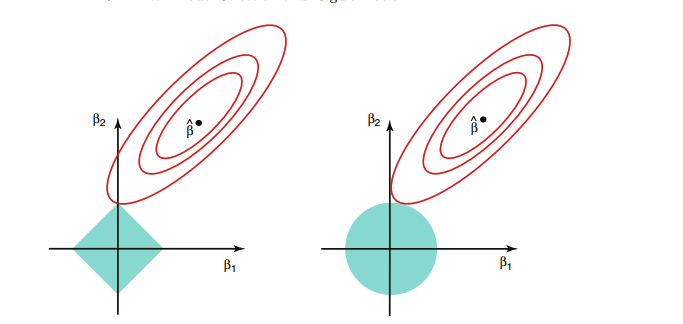
\includegraphics[width=\textwidth]{feature-selection1.png}
    \caption{Illustration of two dimensional case of estimation for the lasso
    (left) and the ridge regression (right)}
    \label{fig:feature-selection}
    \source{\textcite{james2013introduction}}
\end{figure}

\subsubsection*{Selecting the Tuning Parameter}

Choosing an optimized value of tuning parameter $\lambda$ is critical when
implementing the ridge and the lasso regression.
We do not want to choose $\lambda$ too small due to the low restriction. On the
other hand, when $\lambda$ is very large, the restriction is more substantial
than it is desired. We handle the problem of the optimal value of  by using a
cross-validation technique. \textcite{efron1994introduction} introduce the algorithm, which describes
the procedure of cross-validation.

\begin{algorithm}[H]
\setstretch{1.35}
\SetAlgoLined
\renewcommand{\labelenumi}{(\Roman{enumi})}
Split the data into K roughly equal-sized parts.

For the $k^{th}$ part, fit the model to the other K − 1 parts of the data, and
calculate the mean squared error of the fitted model when predicting the
$k^{th}$ part of the data.

Repeat step 2 for k = 1, 2, . . . , K and average the K estimates of mean
squared error $MSE_1$, $MSE_2$,..., $MSE_k$.

For each tuning parameter value $\lambda$, compute the average error over all
folds \[CV_{(k)} = \frac{1}{k} \sum_{i=1}^{k} MSE_i\]

 \caption{K-Fold Cross Validation}
\end{algorithm}


We choose a grid of $\lambda$ values and calculate the cross-validation error
for each value of $\lambda$. We then select the tuning parameter value for which
the cross-validation error is smallest.

\subsection{Boosting}

All the approaches reviewed so far suffer from the fact that they use a single
model for predicting the response variable. Hence the ability to choose a
suitable model is crucial to have any chance to obtain good results.
Machine Learning practitioners have to consider many factors such as
the quantity of data, the dimensionality of the space, and distribution
hypothesis to find a high predictive power model.

Boosting, on the other hand, is an an ensemble technique in which several weak
models such as decision trees  are combined to achieve a stronger one.The
general idea of most boosting methods is to train predictors sequentially, each
trying to correct its prede‐ cessor.

\subsubsection*{Regression Trees}

Regression Tree is a type of decision trees  used to predict continuous
numeric values (e.g. the price of a house, or a patient's length of stay in a
hospital). In a regression tree, each leaf represenet a numeric value.

A regression tree is recursively constructed through a binary partitioning
process. We first select the predictor  and the cut point s such that splitting
the predictor space into the two regions (S1 = {${X|X_j <s}$} and S2 = {${X|X_j
> s}$}) such that the overall sums of squares error are minimized:

\begin{eqnarray}
  \textrm{SSE} = \sum_{i\in S_1}^{n}(y-\bar{y_1})^2 + \sum_{i \in S_2}^{n}(y-\bar{y_2})^2
\end{eqnarray}


where $\hat{y_1}$ and  $\hat{y_1}$ are the mean response for  training set within groups
S1 and S2, respectively.

We repeat the process, looking for the best predictor and best cutpoint to split
the data further to minimize the sums of squares errors within each group. The
recursive partitioning of the data continues until a stopping criterion reached
for instance, we may continue until no region contains more than 20
observations.
We predict the response for a given test data point using the average value of
the training observations in the group to which that test observation belongs.



\subsubsection*{Gradient Boosting}

While having an advantage of being easily be visualized and understood, the main
downside of decision trees is that they tend to overfit and provide poor
generalization performance. Therefore, in most applications, the ensemble
methods such as boosting are usually used in place of a single decision tree.

The underlying idea behind ensemble learning is that by aggregating the
predictions of a group of predictors (such as classifier or regressors) we will
ofter get better predictons than the best individual predictor (\textit{wisdom of the
crowd}).
According to ensemble learning theory, weak learners are models that perform not
so well by themselves either because they have a high bias or because they have
too much variance. Then the idea of ensemble methods is to reduce bias and/or
variance of such weak learners by combining several of them together to create a
strong leader that achieves better predictive performance.

Boosting refers to any ensemble method for primarily reducing bias, and also
variance by combining several weak learners into  a strong learner.  Being
mainly focused at reducing bias, the base learners that are often considered for
boosting are models with low variance but high bias such as shallow decision
trees with only a few depths.
Another reason for using shallow trees in boosting is that it makes the model
smaller in terms of memory and makes prediction faster.

While there are many boosting methods available, in this study, we focus on
Gradient boosting trees and its high-performance implementation, XGBoost. In
gradient boosting trees,  regression trees are chosen  as the base learners.

\textcite{kuhn2013applied} illustrate the Gradient Boosting for
Regression algorithm as followed:

\begin{algorithm}[H]
\setstretch{1.35}
\SetAlgoLined

\renewcommand{\labelenumi}{(\Roman{enumi})}
Select tree depth, D, and number of iterations, K

Compute the average response, $\bar{y}$, and use this as initial predicted value
for each observation in the training set.

\For{$k\gets0$ \KwTo $K$ }{
    Compute the residual, the difference between observed value and the
    \textit{current} predicted value, for each observation.

    Fit a regression tree of depth, D, using the residuals as the response.

    Predict each observation using regression fit in the previous step.

    Update the predicted value of each observation by adding the previous
    iteration's predicted value to the predicted value generated in the previous
    step.

    }
 \caption{Simple Gradient Boosting for Regression}
\end{algorithm}

We can find the the optimal value of tree depth (D) and the number of
iterations (K) by using cross-validation techniques.

\subsubsection*{XGBoost}

XGBoost is an end-to-end tree boosting system developed by
\textcite{chen2016xgboost} based on a
gradient boosting framework.  XGBoost has been shown to provide state-of-the-art
results for diverse problems, including web text classification, customer
behavior prediction, motion detection, and malware classification
\parencite{chen2016xgboost}.

\textcite{nielsen2016tree} shows some features of XGBoost that make it stand out
of from the rest of other gradient boosting algorithms. That is:
\begin{itemize}
    \item Clever penalization of trees
    \item A proportional shrinking of leaf nodes
    \item Newton Boosting
    \item Extra randomization parameter
    \item Implementation on single, distributed systems and out-of-core computation
\end{itemize}

Besides these superior features, there are other reasons why XGBoost is getting
popular in the machine learning community:
\begin{itemize}
    \item Can solve a wide range of applications such as regression,
        classification, ranking, and user-defined prediction problems.
    \item Portability: Runs smoothly on Windows, Linux, and OS X.
    \item Languages: Supports all major programming languages, including C++,
        Python, R, Java, Scala, and Julia.
    \item Cloud Integration: Supports AWS, Azure, and Yarn clusters and works
        well with Flink, Spark, and other ecosystems.
\end{itemize}

While XGBoost is suitable for predicting, it does so at the expense of its
interpretability.  As shown in Figure
\ref{fig:flexibility-interpretability-tradeoff}, compared to restrictive models
such as Lasso or Least Squares, Boosting is a highly flexible (complex) approach
that is harder to interpret.

\begin{figure}[H]\centering
    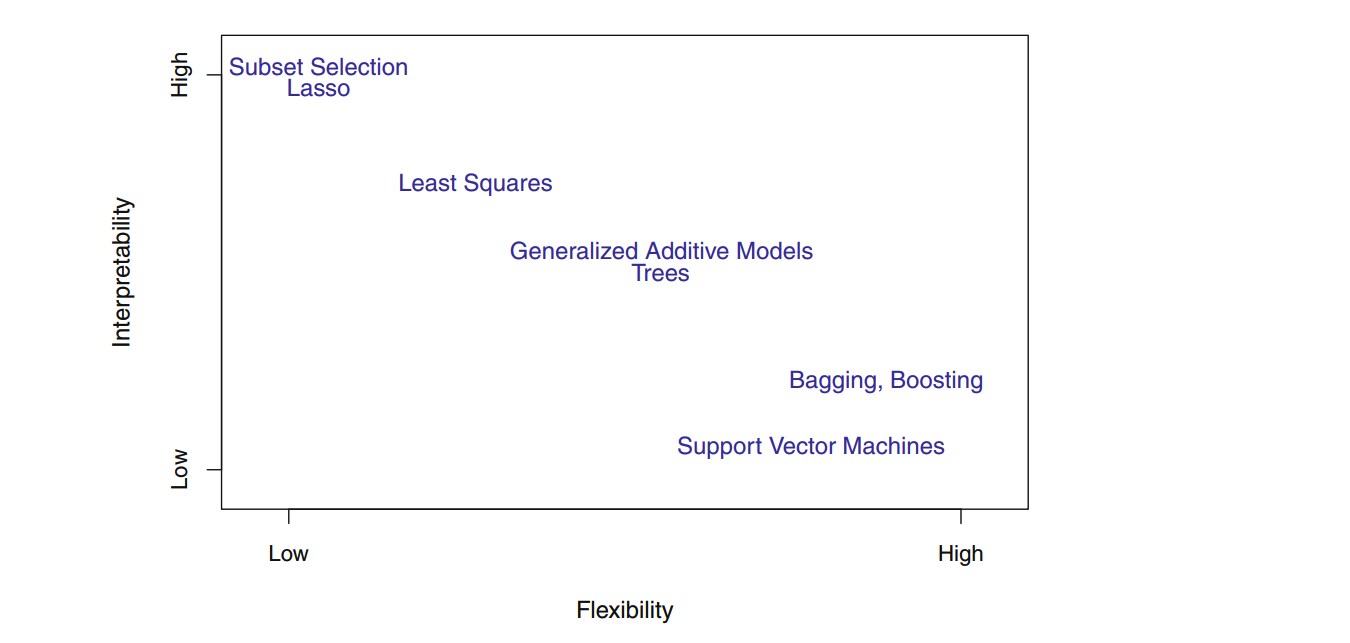
\includegraphics[width=\textwidth]{flexibility-interpretability-tradeoff.png}
    \caption{Interpretability and Flexibility Tradeoff}
    \label{fig:flexibility-interpretability-tradeoff}
    \source{\textcite{james2013introduction}}
\end{figure}


